\documentclass{beamer}

\usepackage{changepage}
\usepackage{hyperref}

\usepackage[skip=0.2\baselineskip]{parskip}

\usepackage{mathrsfs}
\usepackage{caption}
\usepackage{subcaption}
\usepackage{tikz}
\usepackage{makecell}
\usepackage{array,booktabs}
\newcolumntype{C}{>{$\displaystyle}c<{$}}

\setlength\fboxsep{0pt}
\setlength\fboxrule{0pt}

\usepackage{theme/beamerthemepamango-blank}
\usepackage{shortcuts_pm}

\setbeamertemplate{caption}{\raggedright\insertcaption\par}

\addbibresource{references.bib}

%%%%% INFORMATION

\title{Coordinate Descent for Private Composite Empirical Risk Minimization}
\author{
  Paul Mangold \\[1em]
 (Aurélien~Bellet, Marc~Tommasi, Joseph~Salmon)
}
\institute{\textsc{Magnet Seminar}}

\date{February 17th, 2022}

%%%%% DOCUMENT

\begin{document}

%% TITLE PAGE

\begin{notitle}
  \begin{frame}
    \titlepage
  \end{frame}
  \addtocounter{framenumber}{-1}
\end{notitle}

\begin{frame}
  Supervised learning:
  \begin{align*}
    D = \{d_1, \dots, d_n\} \subseteq \cX \times \cY.
  \end{align*}

  \vspace{1em}

  Learn \emph{good parameters} $w \in \RR^p$ for
  \begin{align*}
    h_w : \cX \mapsto \cY.
  \end{align*}
\end{frame}

\begin{frame}
  \vspace{-0.5em}
  {\Huge
    \begin{center}
      Empirical Risk Minimization
    \end{center}
  }
  \vspace{-1.5em}
  \begin{align*}
    \argmin_{w \in \RR^p} F(w) = \underbrace{\frac 1n \sum_{i=1}^n \ell(w; d_i)}_{f(w)}.
  \end{align*}


  Assumptions:

  \vspace{0.5em}

  \begin{itemize}[leftmargin=1em,itemsep=0.5em]
    \Large
  \item $\ell(\cdot; d)$ convex, component-Lipschitz $\forall d\in\cX\times\cY$.
  \item $\ell(\cdot; d_i)$ component-smooth $\forall d_i\in D$.
  \end{itemize}
\end{frame}

\begin{frame}
  $\ell(\cdot; d)$ is component-Lipschitz for $d \in \cX\times\cY$:
  \begin{align*}
    \abs{\ell(w + te_j; d) - \ell(w; d)} \le L_j \abs{t}.
  \end{align*}

  \pause

  \quad $\Rightarrow$ for $w \in \RR^p,$ $\abs{\nabla_j \ell(w; d)} \le L_j$.

  \vspace{1em}
  \pause

  \cbox{
    for $w, w' \in \RR^p$ and $d, d' \in \cX \times \cY$, \\
    $\begin{aligned}
      \abs{\nabla_j \ell(w; d) - \nabla_j \ell(w'; d')} \le 2L_j.
    \end{aligned}$
  }


\end{frame}
\begin{frame}

  $\ell(\cdot; d)$ is component-smooth for $d \in D$:
  \begin{align*}
    \abs{\nabla_j \ell(w + te_j; d) - \nabla_j \ell(w; d)} \le M_j \abs{t}.
  \end{align*}

  \pause

  \vspace{1em}

  \quad $\Rightarrow$ for $w, w' \in \RR^p$,
  {\Large
    \begin{align*}
      f(w') \le f(w) + \scalar{\nabla f(w)}{w' - w} +
      \frac{1}{2}\norm{w'-w}_M^2.
    \end{align*}
    \begin{flushright}
      where $\norm{w}_M^2 = \sum_{j=1}^p M_j w_j^2$.
    \end{flushright}
  }
\end{frame}

\begin{frame}
  \vspace{-0em}
  {\Huge
    \begin{center}
      Composite ERM
    \end{center}
  }
  \vspace{-1.5em}
  \begin{align*}
    \argmin_{w \in \RR^p} F(w) = \underbrace{\frac 1n \sum_{i=1}^n \ell(w; d_i)}_{f(w)} + \psi(w).
  \end{align*}


  Assumptions:

  \vspace{0.5em}

  \begin{itemize}[leftmargin=1em,itemsep=0.5em]
    \Large
  \item $\ell(\cdot; d)$ convex, component-Lipschitz $\forall d\in\cX\times\cY$.
  \item $\ell(\cdot; d_i)$ component-smooth $\forall d_i\in D$.
  \item $\psi(w) = \sum_{j=1}^p \psi_j(w_j)$ convex and separable.
  \end{itemize}
\end{frame}

\begin{frame}
  \begin{center}
    \Huge Example: LASSO
  \end{center}
  \begin{align*}
    \argmin_{w \in \RR^p} \frac{1}{2n} \norm{Xw - y}_2^2 + \lambda \norm{w}_1.
  \end{align*}

  \pause

  \cbox{
    $ \displaystyle M_j = \frac{1}{n} \sum_{i=1}^n \abs{X_{i,j}}^2. $
  }


\end{frame}

\begin{frame}
  \vspace{2em}

  $\emphcolb{\cA} : D \mapsto w$ is
  $(\emphcol{\epsilon}, \emphcol{\delta})$-\emph{Differentially
    Private}
  \begin{align*}
    \prob{\emphcolb{\cA}(D) \in \cS} \le e^{\emphcol{\epsilon}} \prob{\emphcolb{\cA}(D') \in \cS} + \emphcol{\delta}.
  \end{align*}

  \vspace{1em}

  \begin{flushright}
    ($D$ and $D'$ differ on one element.)
  \end{flushright}

  \smalllongcite{dwork2006Differential}
\end{frame}

\begin{frame}
  \vspace{2em}

  \emph{Differentially Private} Composite ERM:
  \begin{align*}
    & \argmin_{w \in \RR^p}  F(w) = f(w) + \psi(w)\\
    & \qquad \text{such that $w$ is $(\epsilon, \delta)$-DP.}
  \end{align*}

  \smalllongcite{chaudhuri2011Differentially}
\end{frame}

\begin{frame}
  \Huge\centering
  Solving DP-ERM?

  \resizebox{5cm}{!}{
    \begin{minipage}{1.0\linewidth}
      \begin{align*}
        & \argmin_{w \in \RR^p} F(w) = f(w) + \psi(w)\\
        & \qquad \text{such that $w$ is $(\epsilon, \delta)$-DP.}
      \end{align*}
    \end{minipage}
  }

  \vspace{1em}
  \pause
  \Large
  The classical: DP-SGD. \pause \\
  The challenger: DP-CD.
\end{frame}

\begin{frame}
  \vspace{2em}

  \only<2>{Private }Stochastic Gradient Descent
  \begin{align*}
    w^{t+1} = \prox_{\eta\psi}\left(w^t - \eta
    \only<1>{\emphcol{\xi}}
    \only<2>{\left( \emphcol{\xi} + \emphcolb{\cN(\sigma^2\bbI)} \right)}\right),
  \end{align*}

  where $\expec{}{\emphcol{\xi}} = \nabla f(w^t)$.

  \vspace{-0.5em}
  \only<1>{\longcite{beck2009Fast,mishchenko2021Proximal}}
  \only<2>{\longcite{bassily2014Differentially,wang2017Differentially}}
\end{frame}


\begin{frame}
  \vspace{2em}

  \only<2>{Private }Coordinate Descent
  \begin{align*}
    \!w^{t+1}_{j}\!\! =\!
    \prox_{\eta_j\psi_j}\!
    \left(w^t_{j} - \eta_{j}\!
    \only<1>{ \emphcol{\nabla_{j} f(w^t)} }
    \only<2>{ \left( \emphcol{\nabla_{j} f(w^t)}
    \!+\! \emphcolb{\cN(\sigma_{j}^2)} \right) \! }\right),
  \end{align*}

  \vspace{1.5em}

  \begin{flushright}
    where $j \in \{1, \dots, p\}$ is chosen randomly.
  \end{flushright}

  \only<1>{\longcite{richtarik2014Iteration}}
  \only<2>{\fbox{\phantom{\longcite{richtarik2014Iteration}}}}
\end{frame}

\begin{frame}
  DP-SGD:
  \begin{align*}
    w^{t+1} = \prox_{\emphcolc{\eta}\emphcol{\psi}}\left(w^t - \emphcolc{\eta} \left( \emphcol{\xi}
    + \emphcolb{\cN(\sigma^2\bbI)} \right)\right),
  \end{align*}

  \begin{flushright}
    with $\expec{}{\xi} = \nabla f(w^t)$.
  \end{flushright}

  DP-CD:
  \begin{align*}
    \!\!w^{t+1}_{j}\!\! =\!
    \prox_{\emphcolc{\eta_j}\emphcol{\psi_j}}\!
    \left(w^t_{j} - \emphcolc{\eta_{j}}\!
    \left( \emphcol{\nabla_{j} f(w^t)}
    \!+\! \emphcolb{\cN(\sigma_{j}^2)} \right)\!\right).
  \end{align*}
\end{frame}


\begin{frame}
  \vspace{-0.5em}
  \only<5>{\vspace{2.075em}}
  \only<6>{\vspace{0.225em}}
  \begin{table}
    {\setlength{\tabcolsep}{0.4em}
      \centering
      \begin{tabular}{ccc}
        & DP-SGD
        & DP-CD \\
        \hline
        \hline
        \makecell{Assumptions \\[-0.5em] on $f$}
        & \normalsize
          \makecell{
          \normalsize $\Lambda$-Lipschitz \\
          \normalsize $\beta$-smooth
        }
        & \normalsize
          \makecell{
          \normalsize $L$-comp.-Lipschitz \\
          \normalsize $M$-comp.-smooth \\
          }
        \\[0.5em]
        \hline
        \\[-1.5em]
        % \pause
        % Iterations
        % \pause
        % & $T \propto n$
        % \pause
        % & $T \propto p$
        % \pause \\[0.5em]
        Step sizes
        \only<2-6>{
        & $\eta \propto 1/\beta$
          \only<3-6>{
        & $\eta_j \propto 1/M_j$
          \only<4-6>{\\[0.5em]
        Noise scale
        \only<5-6>{
        & $\sigma^2 = O\Big(\frac{\emphcol{\Lambda^2}T}{n^2\epsilon^2}\Big)$
           \only<6-6>{
        & $\sigma_j^2 = O\Big(\frac{\emphcol{L_j^2} T}{n^2\epsilon^2}\Big)$
        }}}}}
      \end{tabular}
    }
  \end{table}
  \only<5>{\vspace{1em}
    Since $\displaystyle\sup_{d,d'} \norm{\nabla \ell(\cdot;d) - \nabla\ell(\cdot;d')}_2 \le 2\Lambda$.
  }
  \only<6>{\vspace{1em}
    Since $\displaystyle\sup_{d,d'} \abs{\nabla_j \ell(\cdot;d) - \nabla_j\ell(\cdot;d')} \le 2L_j$.
  }
\end{frame}

\begin{frame}
  \vspace{1em}

  \begin{center}
    \Huge What about this $O\Big( \cdot \Big)$?
  \end{center}

  \vspace{1em}

  DP-SGD: sampling rate $q \le 1$,

  {\tiny
    \begin{align*}
      \!\!\!\epsilon & \le \frac{1}{\alpha - 1} \log\left(
                       \frac{1}{2}\sum_{k=0}^\infty \binom{\alpha}{k} (1-q)^{\alpha-k}q^k \exp\left(\frac{k^2-k}{2\sigma^2} \right) \!\!\left( \erfc\!\left(\frac{z_1-k}{\sqrt{2}\sigma}\right) \!+\! \erfc\!\left(\frac{k-z_1}{\sqrt{2}\sigma} \right) \right)
                       \right)
                       + \frac{\log(1/\delta)}{\alpha - 1}.
    \end{align*}
  }
  \pause

  DP-CD: \emph{not needed!}

  \vspace{-1.5em}

  \smalllongcite{mironov2019Renyi}
\end{frame}

\begin{frame}
  \vspace{1em}

  \begin{center}
    \Huge Utility?
  \end{center}

  \begin{align*}
    \expec{}{F(w^T)-F^*} \le ~?
  \end{align*}
\end{frame}

\begin{frame}
  \begin{center}
    \Huge \textit{Ad hoc} dual norms.
  \end{center}

  \Large
  \begin{align*}
    \norm{w}_{M} = \sqrt{ \sum_{j=1}^p M_j w_j^2 }
    \qquad
    \norm{w}_{M^{-1}} = \sqrt{ \sum_{j=1}^p \frac{1}{M_j} w_j^2 }.
  \end{align*}
\end{frame}

\begin{frame}
  \vspace{3em}
  \begin{table}
    {\setlength{\tabcolsep}{0.3em}
      \centering
      \begin{tabular}{ccc}
        & DP-SGD
        & DP-CD \\
        \hline
        \hline
        \\[-1.7em]
        \Large \makecell{Assumptions \\[-0.5em] \normalsize on $f$}
        & \normalsize
          \makecell{
          \normalsize convex \\[0.5em]
          \normalsize $\Lambda$-Lipschitz \\[0.5em]
          \normalsize $\beta$-smooth
        }
        & \normalsize
          \makecell{
          \normalsize convex \\[0.5em]
          \normalsize $L$-comp.-Lipschitz \\[0.5em]
          \normalsize $M$-comp.-smooth
        }
        \\[1em]
        \hline
        \\[-1.5em]
        \Large\makecell{Utility \\[-0.5em] \scriptsize ($\expec{}{F(w)-F^*} \le ...$)}
        & \only<2,3>{$O\Big( \frac{\emphcol{\Lambda R_I}\sqrt{p} }{n\epsilon} \Big)$}
        & \only<3>{$O\Big(\frac{ \emphcol{\norm{L}_{M^{-1}} R_M} \sqrt{p} }{n\epsilon}\Big)$}
      \end{tabular}
    }
  \end{table}

  \vspace{2em}
  \only<1>{\vspace{1em}}

  \large \only<2,3>{Where}\scriptsize
  \begin{tabular}{l}
    \large \only<3>{$\norm{L}_{M^{-1}} = (\sum_{j=1}^p L^2_j / M_j)^{1/2}$,} \\
    \large \only<2,3>{$R_I^2 = \max( F(w^0) - F(w^*), \norm{w^0 - w^*}_2^2)$\only<2>{.}\only<3>{,}} \\
    \large \only<3>{$R_M^2 = \max( F(w^0) - F(w^*), \norm{w^0 - w^*}_M^2)$.}
  \end{tabular}
\end{frame}


\begin{frame}
  \vspace{3em}
  \begin{table}
    {\setlength{\tabcolsep}{0.3em}
      \centering
      \begin{tabular}{ccc}
        & DP-SGD
        & DP-CD \\
        \hline
        \hline
        \\[-1.7em]
        \Large \makecell{Assumptions \\[-0.5em] \normalsize on $f$}
        & \normalsize
          \makecell{
          \normalsize $\mu_I$-strongly-convex \\ \wrt $\norm{\cdot}_2$ \\[0.5em]
          \normalsize $\Lambda$-Lipschitz \\[0.5em]
          \normalsize $\beta$-smooth
        }
        & \normalsize
          \makecell{
          \normalsize $\mu_M$-strongly-convex \\ \wrt $\norm{\cdot}_M$ \\[0.5em]
          \normalsize $L$-comp.-Lipschitz \\[0.5em]
          \normalsize $M$-comp.-smooth
        }
        \\[1em]
        \hline
        \\[-1.5em]
        \Large\makecell{Utility \\[-0.5em] \scriptsize ($\expec{}{F(w)-F^*} \le ...$)}
        & \only<2,3>{$O\Big(\frac{\emphcol{\Lambda^2} p }{\emphcol{\mu_I}n^2\epsilon^2} \Big)$}
        & \only<3>{$O\Big(\frac{\emphcol{\norm{L}_{M^{-1}}^2}p}{\emphcol{\mu_M}n^2\epsilon^2}\Big)$}
      \end{tabular}
    }
  \end{table}

  \vspace{3em}

  \only<3>{
  \large Where\scriptsize
  \begin{tabular}{l}
    \large $\norm{L}_{M^{-1}} = (\sum_{j=1}^p L^2_j / M_j)^{1/2}$.
  \end{tabular}
  }
\end{frame}

\begin{frame}

  \vspace{2em}
  {
    \Huge\centering
    CD vs. SGD: Who wins?
  }
  \vspace{1em}


  Balanced $M_j$'s:

    {\centering $\rightarrow$ DP-SGD up to $\emphcol{p}$ times better.}
\end{frame}

\begin{frame}

  \vspace{2em}
  {
    \Huge\centering
    CD vs. SGD: Who wins?
  }
  \vspace{1em}

  Imbalanced $M_j$'s:

  {\centering $\rightarrow$ DP-CD up to $\emphcol{\frac{\max_j M_j}{\min_j M_j}}$ times better.}
  \vspace{1em}

\end{frame}

\begin{frame}
  \vspace{2em}
  \Huge\centering
  Practical Comments.

  \vspace{1em}

  \LARGE
  \begin{itemize}
  \item Gradient Clipping.
  \item Hyperparameters.
  \item Private Smoothness Constants?
  \end{itemize}
\end{frame}

\begin{frame}
  \begin{align*}
    \displaystyle \abs{\nabla_j \ell(w; d)} \le L_j \text{\quad for $d \in \cX\times\cY$}.
  \end{align*}

  \pause

  \begin{align*}
    \Rightarrow \sigma_j^2 = O\left( \frac{\emphcol{L_j}^2 T}{n^2\epsilon^2} \right).
  \end{align*}
\end{frame}

\begin{frame}
  {\Huge
    \begin{center}
      Clip!
    \end{center}
  }
  \vspace{-0.5em}
  {\Large
    \begin{align*}
      \!\!\!\!\clip(\nabla_j \ell(w;d), C_{\emphcol{j}}) = \twopartdef
      {\pm C_{\emphcol{j}}}{\text{if }\abs{\nabla_j \ell(w;d)} > C_{\emphcol{j}},}
      {\nabla_j \ell(w; d)}{\text{otherwise.}}
    \end{align*}
  }

  \pause

  \vspace{-1em}

  \cbox {
    $\displaystyle \abs{\clip(\nabla_j \ell, C_{\emphcol{j}})} \le C_{\emphcol{j}}
    \Rightarrow \sigma_j = O\left( \frac{\emphcol{C_j}^2 T}{n^2\epsilon^2}\right)
    $.
  }

\end{frame}


\begin{frame}
  \vspace{2em}
  \begin{table}
    \centering
    \begin{tabular}{c|cc}
      & DP-SGD
      & DP-CD
      \\
      \hline
      \hline
      \\[-1em]
      Clipping
      & $C$
      & \only<2>{$C_j = \sqrt{\frac{M_j}{\tr(M)}} C$} \\[1em]
      Step sizes
      & $\eta = \gamma/\beta$
      & \only<2>{$\eta_j = \gamma/M_j$}
    \end{tabular}
  \end{table}
\end{frame}


\begin{frame}
  \vspace{-1em}
    % \Huge
    % Smoothness Constants...
  \begin{align*}
    & \argmin_{w \in \RR^p} \overbrace{\frac 1n \sum_{i=1}^n
      \underbrace{\ell(w, d_i)}_{M^{(i)}\text{-comp-smooth}}}^{f(w)} + \psi(w)
  \end{align*}

  \pause

  \vspace{0.5em}
  \cbox {
    $\displaystyle M_j = \frac{1}{n} \sum_{i=1}^n M_j^{(i)}.$
  }
\end{frame}


\begin{frame}
  \vspace{-1em}
    % \Huge
    % Smoothness Constants...
  \begin{align*}
    & \argmin_{w \in \RR^p} \overbrace{\frac 1n \sum_{i=1}^n
      \underbrace{(X_{i,:}^Tw - y_i)^2}_{M^{(i)}\text{-comp-smooth}}}^{f(w)} + \lambda\norm{w}_1
  \end{align*}

  \cbox{
    $ \displaystyle M_j = \frac{1}{n} \sum_{i=1}^n \abs{X_{i,j}}^2. $
  }

  \pause

  \begin{center}
    Remark: standardized data $\rightarrow$ $M_j=1$.
  \end{center}
\end{frame}




\begin{frame}
  \vspace{-1em}
  % \begin{center}
  %   \Huge
  %   \emph{Private} Smoothness Constants!
  %   \resizebox{7cm}{!}{
  %   \begin{minipage}{1.0\linewidth}
  \begin{align*}
    & \argmin_{w \in \RR^p} \overbrace{\frac 1n \sum_{i=1}^n
      \underbrace{\ell(w, d_i)}_{M^{(i)}\text{-comp-smooth}}}^{f(w)} + \psi(w)
  \end{align*}
  % \end{minipage}
  % }
  % \end{center}

  \vspace{0.5em}

  Let $\epsilon' \le \epsilon$ (\eg $\epsilon' = 0.1 \epsilon$).

  \cbox {
    \Large
    $\displaystyle
    \!\!M_j^{priv}\!\! =\! \frac{1}{n} \sum_{i=1}^n M_j^{(i)} + \Lap\left(\frac{p \cdot \emphcol{\max_i M_j^{(i)}}}{n \epsilon'}\right).
    $
  }
\end{frame}

\begin{frame}
  \vspace{1em}
%  \begin{center}
%    \Huge
%    \emph{Private} Smoothness Constants!
%    \resizebox{7cm}{!}{
%      \begin{minipage}{1.0\linewidth}
    \begin{minipage}{1.0\linewidth}
      \begin{align*}
        & \argmin_{w \in \RR^p} \overbrace{\frac 1n \sum_{i=1}^n
          f_i(w)}^{f(w)} + \psi(w)
      \end{align*}
    \end{minipage}
% \end{minipage}
%    }
%  \end{center}

  \vspace{0.5em}

  Let $\epsilon' \le \epsilon$ (\eg $\epsilon' = 0.1 \epsilon$).

  \cbox {
    \Large
    $\displaystyle
    \!\!M_j^{priv}\!\! =\! \frac{1}{n} \sum_{i=1}^n \clip(M_j^{(i)}, \emphcol{b_j}) + \Lap\left(\frac{p \cdot \emphcol{b_j}}{n \epsilon'}\right).
    $
  }
\end{frame}

\begin{frame}
  \begin{center}
    \Huge Experiments.
  \end{center}

  \begin{itemize}[itemsep=0.5em]
  \item On logistic regression and LASSO.

  \item Tune
    $\left\{\rule{0cm}{2.5em}\right.
      \begin{tabular}{l}
        step size, \\
        clipping threshold,\\
        number of iterations.
      \end{tabular}
      $

    \item Average over $10$ runs.

  \end{itemize}
\end{frame}

\begin{frame}
  \begin{center}
    \Huge Imbalanced Dataset
  \end{center}

  \pause

  \vspace{1em}
  \begin{minipage}{0.5\linewidth}
    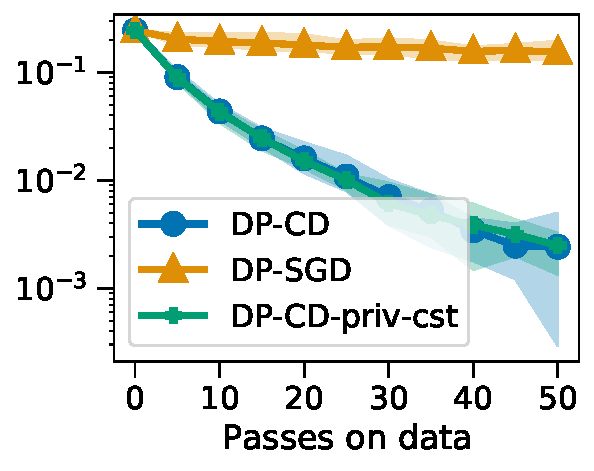
\includegraphics[width=\linewidth]{images/optimization_electricity_raw.pdf}%
    \begin{center}
      \normalsize
      \textsc{Electricity (raw)} \\
      $n=45,312$~~$p=8$ \\
      Logistic Regression
    \end{center}
  \end{minipage}%
  \begin{minipage}{0.5\linewidth}
    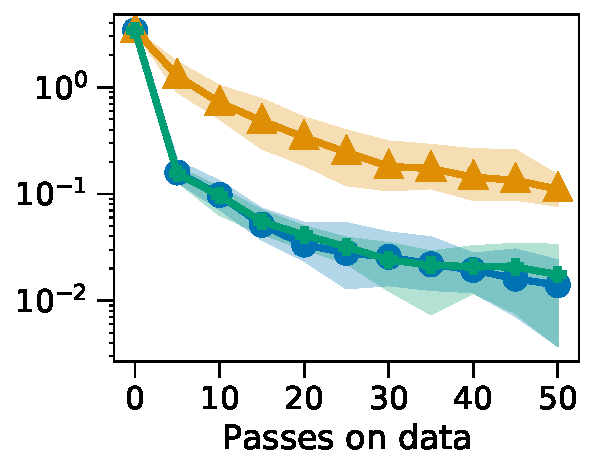
\includegraphics[width=\linewidth]{images/optimization_california_raw.pdf}%
    \begin{center}
      \normalsize
      \textsc{California (raw)} \\
      $n=20,640$~~$p=8$ \\
      LASSO
    \end{center}
  \end{minipage}

  \vspace{1em}

  \begin{center}
    \Large $\epsilon = 1$, $\delta = 1 / n^2$.
  \end{center}
\end{frame}

\begin{frame}
  \begin{center}
    \Huge Balanced Dataset
  \end{center}

  \pause

  \vspace{1em}
  \begin{minipage}{0.5\linewidth}
    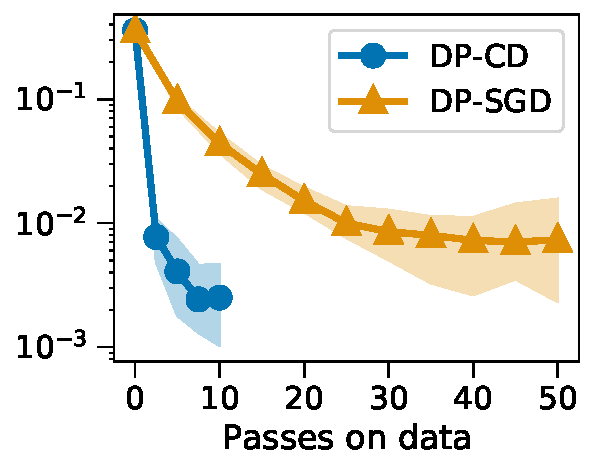
\includegraphics[width=\linewidth]{images/optimization_electricity_norm.pdf}%
    \begin{center}
      \normalsize
      \textsc{Electricity (scaled)} \\
      $n=45,312$~~$p=8$ \\
      Logistic Regression
    \end{center}
  \end{minipage}%
  \begin{minipage}{0.5\linewidth}
    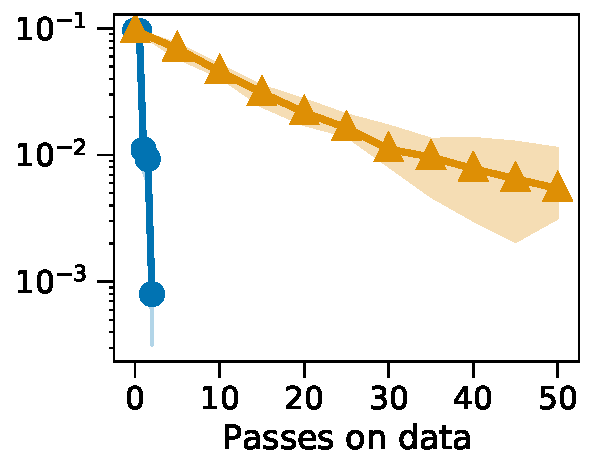
\includegraphics[width=\linewidth]{images/optimization_california_norm.pdf}%
    \begin{center}
      \normalsize
      \textsc{California (scaled)} \\
      $n=20,640$~~$p=8$ \\
      LASSO
    \end{center}
  \end{minipage}

  \vspace{1em}

  \begin{center}
    \Large $\epsilon = 1$, $\delta = 1 / n^2$.
  \end{center}
\end{frame}


\begin{frame}
  \begin{center}
    \Huge Higher dimension
  \end{center}

  \pause

  \vspace{1em}

  \begin{minipage}{\linewidth}
    \centering
    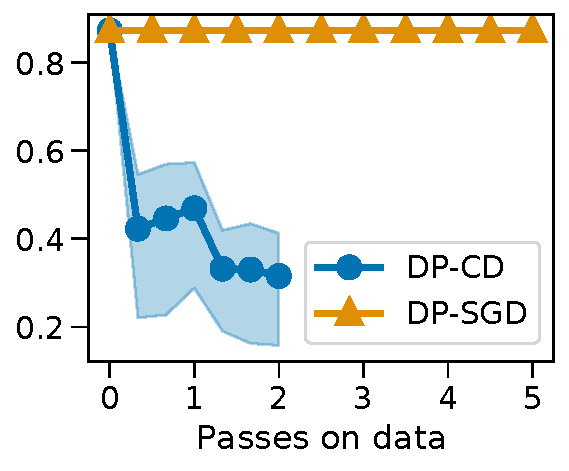
\includegraphics[width=0.5\linewidth]{images/optimization_lasso.pdf}
  \end{minipage}
  \begin{center}
    \normalsize
    \textsc{Sparse Solution} \\
    $n=1,000$~~$p=1,000$ \\
    LASSO
  \end{center}

  \vspace{0.5em}

  \begin{center}
    \Large $\epsilon = 10$, $\delta = 1 / n^2$ and $\norm{w^*}_0 = 10$.
  \end{center}
\end{frame}

\begin{frame}
  { \Huge
  \begin{center}
    Partial Conclusion.
  \end{center}
  }
  \begin{itemize}
  \item Partial gradients without amplification.
  \item Large learning rates.
  \item Good practical performance.
  \end{itemize}
\end{frame}

\begin{frame}

  \vspace{2em}

  {\Huge\centering
    Is DP-CD optimal? \only<1>{}\only<2>{Kind of.}\only<3>{Yes, if...}
  }

  \vspace{1em}
  \only<2,3>{
    \begin{tabular}{c|cc}
      \Large Loss
      & \Large \makecell{Convex \\ $L$-comp.-Lipschitz}
      & \Large \makecell{Strongly-Convex \\ $L$-comp.-Lipschitz} \\
      \hline
      \hline
      \\[-1.3em]
      \Large\makecell{Utility \\[-0.5em] \scriptsize ($\expec{}{F(w)-F^*} \ge ...$)}
      & \Large $\Omega\Big(\only<2>{\emphcol{\frac{L_{\min}}{L_{\max}}}} \frac{\norm{L}_2 \norm{w^*}_2 \sqrt{p}}{n \epsilon}\Big)$
      & \Large $\Omega\Big(\only<2>{\emphcol{\frac{L_{\min}^2}{L_{\max}^2}}} \frac{\norm{L}_2^2 p}{\mu_I n^2 \epsilon^2}\Big)$
    \end{tabular}

    \vspace{2em}

    \only<2>{\vspace{1em}}
    \only<3>{
      \begin{center}
        \Large If $\sum_{j \in \cS} L_j^2 = \Omega(\norm{L}_2^2)$ for $\cS$ with $\card{\cS} \ge \frac{p}{75}$.
      \end{center}
    }
  }
\end{frame}


\begin{frame}

  \vspace{4em}
  {\Huge
    \begin{center}
      Thank you! Questions? :)
    \end{center}
  }

  \vspace{3em}

  See our paper:

  \vspace{-1em}

  \smalllongcite{mangold2021Differentially}

\end{frame}
% Plan
% - empirical risk minimization
% - *private*

\end{document}
%%% Local Variables:
%%% mode: latex
%%% TeX-master: t
%%% End:
